\documentclass[11pt,a4paper]{article}

% ── Geometry ──────────────────────────────────────────────────────────────────
\usepackage[top=2cm,bottom=2cm,left=2cm,right=2cm,headheight=14pt]{geometry}

% ── Encoding & fonts ──────────────────────────────────────────────────────────
\usepackage[T1]{fontenc}
\usepackage[utf8]{inputenc}
\usepackage{lmodern}

% ── Colors ────────────────────────────────────────────────────────────────────
\usepackage{xcolor}
\definecolor{MainBlack}{HTML}{222222}
\definecolor{DimGray}{HTML}{666666}
\definecolor{ToneGrayBg}{HTML}{F5F5F5}
\definecolor{ToneGrayFrame}{HTML}{333333}
\definecolor{ToneBlueBg}{HTML}{F0F7FF}
\definecolor{ToneBlueFrame}{HTML}{2E5A88}
\definecolor{ToneRedBg}{HTML}{FFF5F5}
\definecolor{ToneRedFrame}{HTML}{A33333}
\definecolor{AxisRed}{HTML}{C8102E}
\definecolor{AxisBlue}{HTML}{1A5276}
\definecolor{AxisGreen}{HTML}{1D8348}
\definecolor{ArmGray}{HTML}{888888}

% ── Math & Units ──────────────────────────────────────────────────────────────
\usepackage{amsmath}
\usepackage{siunitx}
\sisetup{per-mode = symbol, range-phrase = { to }, range-units = single}

% ── Tables ────────────────────────────────────────────────────────────────────
\usepackage{booktabs}
\usepackage{array}
\usepackage{tabularx}
\usepackage[table]{xcolor}

% ── Code listings ─────────────────────────────────────────────────────────────
\usepackage{listings}
\lstdefinestyle{PythonStyle}{
  language=Python, basicstyle=\ttfamily\small,
  keywordstyle=\bfseries, commentstyle=\color{DimGray}\itshape,
  stringstyle=\color{DimGray}, numberstyle=\tiny\color{DimGray},
  backgroundcolor=\color{ToneGrayBg}, frame=single,
  rulecolor=\color{ToneGrayFrame!20}, breaklines=true, tabsize=4,
  showstringspaces=false, xleftmargin=5pt,
}
\lstdefinestyle{BashStyle}{
  language=bash, basicstyle=\ttfamily\small, keywordstyle=\bfseries,
  backgroundcolor=\color{black!5}, frame=leftline, framerule=2pt,
  rulecolor=\color{ToneGrayFrame}, numbers=none, breaklines=true,
  tabsize=4, showstringspaces=false, xleftmargin=10pt,
}

% ── Boxes ─────────────────────────────────────────────────────────────────────
\usepackage[most]{tcolorbox}
\tcbset{
  accentbox/.style={enhanced, breakable, sharp corners, boxrule=0pt,
    leftrule=3pt, left=10pt, right=10pt, top=8pt, bottom=8pt,
    fonttitle=\bfseries\small, attach title to upper,
    after title={\par\smallskip\hrule\smallskip}},
  setupbox/.style={accentbox, colback=ToneGrayBg, colframe=ToneGrayFrame,
    coltitle=ToneGrayFrame},
  safetybox/.style={accentbox, colback=ToneRedBg, colframe=ToneRedFrame,
    coltitle=ToneRedFrame},
  infobox/.style={accentbox, colback=ToneBlueBg, colframe=ToneBlueFrame,
    coltitle=ToneBlueFrame},
  outcomebox/.style={accentbox, colback=white, colframe=MainBlack,
    coltitle=MainBlack, title={Lab Outcomes}},
}

% ── Lists ─────────────────────────────────────────────────────────────────────
\usepackage{enumitem}
\setlist{noitemsep, topsep=3pt}

% ── TikZ ──────────────────────────────────────────────────────────────────────
\usepackage{tikz}
\usetikzlibrary{arrows.meta, calc, angles, quotes}

% ── Headers & footers ─────────────────────────────────────────────────────────
\usepackage{fancyhdr}
\pagestyle{fancy}
\fancyhf{}
\renewcommand{\headrulewidth}{0.4pt}
\renewcommand{\footrulewidth}{0.4pt}
\lhead{\textbf{ME403 -- Introduction to Robotics}}
\rhead{\textit{Lab 01: Forward Kinematics}}
\lfoot{\small Sabanci University, Spring 2025-26}
\rfoot{\small Page \thepage}

% ── Section formatting ────────────────────────────────────────────────────────
\usepackage{titlesec}
\titleformat{\section}{\large\bfseries}{\thesection.}{0.5em}{}
  [\rule{\linewidth}{0.8pt}]
\titleformat{\subsection}{\normalsize\bfseries}{\thesubsection.}{0.5em}{}
\titlespacing*{\section}{0pt}{18pt}{8pt}
\titlespacing*{\subsection}{0pt}{12pt}{6pt}

% ── Hyperlinks ────────────────────────────────────────────────────────────────
\usepackage{hyperref}
\hypersetup{colorlinks=true, linkcolor=MainBlack,
  urlcolor=ToneBlueFrame, citecolor=MainBlack}

% ── Misc ──────────────────────────────────────────────────────────────────────
\setlength{\parskip}{6pt}
\setlength{\parindent}{0pt}

% ──────────────────────────────────────────────────────────────────────────────
\begin{document}

% ── Title block ───────────────────────────────────────────────────────────────
\thispagestyle{fancy}
\begin{center}
  \rule{\linewidth}{1.5pt}\\[8pt]
  {\LARGE\bfseries ME403 -- Introduction to Robotics}\\[4pt]
  {\large\bfseries Lab 01: Forward Kinematics}\\[4pt]
  {\normalsize Sabanci University \quad|\quad Spring 2025-26}\\[4pt]
  {\small Prepared by Yunus Emre Danabas for ME403}\\[6pt]
  \rule{\linewidth}{1.5pt}
\end{center}

\vspace{5pt}

\begin{tcolorbox}[outcomebox]
  By the end of this lab, you will be able to:
  \begin{itemize}
    \item Explain the difference between body-frame and absolute joint angles.
    \item Write Python calculation scripts that command the robot without a GUI.
    \item Apply the planar 2R forward kinematics (FK) formula to predict end-effector position.
    \item Execute multi-step joint-space trajectories using a single function call per step.
    \item Compare FK predictions to the robot's reported Cartesian pose and interpret the error.
  \end{itemize}
\end{tcolorbox}

% ──────────────────────────────────────────────────────────────────────────────
\section{Body-Frame Joint Angles}
% ──────────────────────────────────────────────────────────────────────────────

\subsection{What ``body-frame'' means}

A joint angle can be measured in two different ways:
\begin{itemize}
  \item \textbf{Absolute (world-frame):} the angle from a fixed world reference (e.g., from horizontal). The firmware internally uses this convention.
  \item \textbf{Body-frame (relative):} the angle from the previous link's own direction. This is the physically intuitive measurement --- you can check it with a protractor placed on the robot.
\end{itemize}

In this lab you always work with \textbf{body-frame angles} $q = [q_1, q_2, q_3, q_4]$.
The utility functions convert to firmware values automatically.

\subsection{Diagram}

The diagram below shows the key difference.
$q_2$ is the shoulder elevation from horizontal (same in both conventions).
$q_3$ is the elbow angle \emph{from the upper-arm direction} (body-frame) ---
\textbf{not} from horizontal. The absolute elbow angle $\theta_3 = q_2 + q_3$.

\vspace{8pt}
\begin{center}
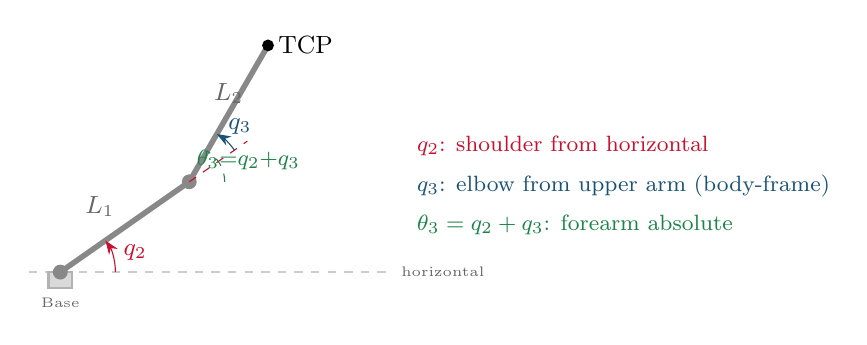
\begin{tikzpicture}[>={Stealth[length=5pt]}, thick]
  % Coordinate definitions (not to scale; illustrative)
  % theta2 = 35 deg, q3_body = 25 deg => theta3 = 60 deg
  % Shoulder at origin, arms length 2 cm each
  \def\thetaA{35}   % shoulder absolute (deg)
  \def\thetaB{60}   % forearm absolute (deg) = 35+25
  \def\Lone{2.0}
  \def\Ltwo{2.0}

  % Computed coordinates
  \coordinate (S) at (0,0);            % shoulder
  \coordinate (E) at ({2.0*cos(\thetaA)}, {2.0*sin(\thetaA)});  % elbow
  \coordinate (T) at ({2.0*cos(\thetaA)+2.0*cos(\thetaB)},
                      {2.0*sin(\thetaA)+2.0*sin(\thetaB)});      % TCP

  % Ground / base
  \draw[gray!40, dashed] (-0.4,0) -- (4.2,0) node[right, font=\tiny, DimGray] {horizontal};
  \filldraw[gray!30] (-0.15,{-0.2}) rectangle (0.15,0);
  \draw[gray!60] (-0.15,-0.2) rectangle (0.15,0);
  \node[font=\tiny, DimGray, below] at (0,-0.2) {Base};

  % Arm links
  \draw[ArmGray, line width=2pt] (S) -- (E);
  \draw[ArmGray, line width=2pt] (E) -- (T);
  \filldraw[ArmGray] (S) circle (0.08);
  \filldraw[ArmGray] (E) circle (0.08);
  \filldraw[black]   (T) circle (0.06) node[right, font=\small] {TCP};

  % q2: angle from horizontal to upper arm (at shoulder)
  \draw[->, AxisRed, thin]
    (0.7,0) arc[start angle=0, end angle=\thetaA, radius=0.7cm];
  \node[AxisRed, font=\small\bfseries] at (0.95,0.25) {$q_2$};

  % Reference line along upper arm direction (for q3 measurement)
  \coordinate (Eref) at ({2.0*cos(\thetaA)+0.9*cos(\thetaA)},
                         {2.0*sin(\thetaA)+0.9*sin(\thetaA)});
  \draw[AxisRed, dashed, thin] (E) -- (Eref);

  % q3: body-frame elbow angle (from upper arm direction to forearm)
  \draw[->, AxisBlue, thin]
    ({2.0*cos(\thetaA)+0.7*cos(\thetaA)},
     {2.0*sin(\thetaA)+0.7*sin(\thetaA)})
    arc[start angle=\thetaA, end angle=\thetaB, radius=0.7cm];
  \node[AxisBlue, font=\small\bfseries]
    at ({2.0*cos(\thetaA)+0.95*cos(47.5)},
        {2.0*sin(\thetaA)+0.95*sin(47.5)}) {$q_3$};

  % theta3: absolute forearm angle (reference arc from horizontal)
  \draw[AxisGreen, dashed, thin]
    ({2.0*cos(\thetaA)+0.45}, {2.0*sin(\thetaA)})
    arc[start angle=0, end angle=\thetaB, radius=0.45cm];
  \node[AxisGreen, font=\footnotesize]
    at ({2.0*cos(\thetaA)+0.75}, {2.0*sin(\thetaA)+0.28}) {$\theta_3{=}q_2{+}q_3$};

  % Labels
  \node[font=\small, DimGray, above left] at ({cos(\thetaA)}, {sin(\thetaA)}) {$L_1$};
  \node[font=\small, DimGray, above] at
    ({2.0*cos(\thetaA)+cos(\thetaB)}, {2.0*sin(\thetaA)+sin(\thetaB)}) {$L_2$};

  % Legend
  \node[AxisRed, font=\footnotesize, anchor=west] at (4.4, 1.6)
    {$q_2$: shoulder from horizontal};
  \node[AxisBlue, font=\footnotesize, anchor=west] at (4.4, 1.1)
    {$q_3$: elbow from upper arm (body-frame)};
  \node[AxisGreen, font=\footnotesize, anchor=west] at (4.4, 0.6)
    {$\theta_3 = q_2+q_3$: forearm absolute};
\end{tikzpicture}
\end{center}
\vspace{4pt}

\subsection{Body-Frame to Firmware Conversion}

The two robots handle the conversion differently because of their internal mechanics.
\texttt{moveMagician()} and \texttt{moveMG400()} perform this conversion for you.

\renewcommand{\arraystretch}{1.3}
\begin{tabularx}{\linewidth}{@{}llXX@{}}
  \toprule
  \textbf{Joint} & \textbf{Body-frame input} & \textbf{Magician firmware} & \textbf{MG400 firmware} \\
  \midrule
  J1 & $q_1$ & $q_1$ & $q_1$ \\
  J2 & $q_2$ & $q_2$ & $q_2$ \\
  J3 & $q_3$ & $q_3$ (quirk: Magician J3 IS body-frame) & $q_2 + q_3$ \\
  J4 & $q_4$ & $q_2 + q_3 + q_4$ & $q_2 + q_3 + q_4$ \\
  \bottomrule
\end{tabularx}

\begin{tcolorbox}[infobox, title={DH Convention (coming in Week 4)}]
  Professional robot software uses the \textbf{Denavit-Hartenberg (DH)} convention to
  systematically assign coordinate frames to each joint. DH parameters give you
  the same geometric insight as body-frame angles but with a standardized notation
  that works for any kinematic chain. You will study DH in Week 4. For now,
  body-frame angles are the physically intuitive equivalent.
\end{tcolorbox}

% ──────────────────────────────────────────────────────────────────────────────
\section{Forward Kinematics Formula}
% ──────────────────────────────────────────────────────────────────────────────

Given body-frame joint angles $q = [q_1, q_2, q_3, q_4]$, the end-effector
Cartesian position is predicted by the \textbf{planar 2R model}:

\begin{align}
  \theta_2 &= q_2 \quad \text{(shoulder absolute angle from horizontal)} \\
  \theta_3 &= q_2 + q_3 \quad \text{(forearm absolute angle from horizontal)} \\[6pt]
  r_{\text{reach}} &= L_1 \cos\theta_2 + L_2 \cos\theta_3 \label{eq:reach}\\
  Z_{\text{tip}} &= Z_{\text{base}} + L_1 \sin\theta_2 + L_2 \sin\theta_3 \label{eq:z}\\[6pt]
  X &= r_{\text{reach}} \cos q_1 \label{eq:x}\\
  Y &= r_{\text{reach}} \sin q_1 \label{eq:y}
\end{align}

where $Z_{\text{base}}$ is the height of the shoulder (J2) pivot above the
mounting surface. Equations~\eqref{eq:reach}--\eqref{eq:y} apply in Python as:

\begin{lstlisting}[style=PythonStyle]
import math
theta2 = math.radians(q[1])
theta3 = math.radians(q[1] + q[2])   # forearm absolute angle
reach  = L1*math.cos(theta2) + L2*math.cos(theta3)
Z_pred = Z_base + L1*math.sin(theta2) + L2*math.sin(theta3)
X_pred = reach * math.cos(math.radians(q[0]))
Y_pred = reach * math.sin(math.radians(q[0]))
\end{lstlisting}

\vspace{4pt}
\begin{tabularx}{\linewidth}{@{}lrrrl@{}}
  \toprule
  \textbf{Robot} & \textbf{$L_1$ (mm)} & \textbf{$L_2$ (mm)} & \textbf{$Z_{\text{base}}$ (mm, nominal)} & \textbf{Notes} \\
  \midrule
  Dobot Magician & 135 & 147 & 103 & Verify: move to $q=[0,0,0,0]$, read $Z$ \\
  DOBOT MG400    & 175 & 175 & 116 & Verify: move to $q=[0,0,0,0]$, read $Z$ \\
  \bottomrule
\end{tabularx}

\begin{tcolorbox}[safetybox, title={Singularity Warning}]
  When $q_2 \approx 0$ and $q_3 \approx 0$, the arm is near-horizontal and the
  Jacobian is degenerate: small joint errors produce large end-effector errors.
  Avoid using these configurations for FK verification tasks.
  Keep $q_2 \in [10^{\circ}, 60^{\circ}]$ and $q_3 \in [0^{\circ}, 40^{\circ}]$ for reliable results.
\end{tcolorbox}

% ──────────────────────────────────────────────────────────────────────────────
\section{API Reference}
% ──────────────────────────────────────────────────────────────────────────────

\subsection*{Magician (\texttt{import utils as U})}

\renewcommand{\arraystretch}{1.3}
\begin{tabularx}{\linewidth}{@{}lX@{}}
  \toprule
  \textbf{Call} & \textbf{Description} \\
  \midrule
  \texttt{bot = U.setup(port=None)} &
    Connect, clear alarms, go home. Returns the \texttt{bot} object. \\
  \texttt{U.moveMagician(bot, q)} &
    Move to body-frame $q=[q_1,q_2,q_3,q_4]$ (degrees). Prints conversion. \\
  \texttt{q = U.get\_joints(bot)} &
    Returns body-frame $(q_1,q_2,q_3,q_4)$ in degrees. \\
  \texttt{x,y,z,r = U.get\_pose(bot)} &
    Returns Cartesian pose (mm / degrees). \\
  \texttt{U.teardown(bot)} &
    Go home and close serial port. Call in \texttt{finally} block. \\
  \midrule
  \texttt{U.L1}, \texttt{U.L2}, \texttt{U.Z\_base} &
    Link lengths and shoulder height constants (mm). \\
  \bottomrule
\end{tabularx}

\vspace{6pt}
\subsection*{MG400 (\texttt{import utils\_mg400 as U})}

\begin{tabularx}{\linewidth}{@{}lX@{}}
  \toprule
  \textbf{Call} & \textbf{Description} \\
  \midrule
  \texttt{db, mv = U.setup(robot=1)} &
    Connect, enable, clear errors, go home. Returns \texttt{(dashboard, move\_api)}. \\
  \texttt{U.moveMG400(mv, q)} &
    Move to body-frame $q=[q_1,q_2,q_3,q_4]$. Prints conversion. \\
  \texttt{q = U.get\_joints(db)} &
    Returns body-frame $(q_1,q_2,q_3,q_4)$ in degrees. \\
  \texttt{x,y,z,r = U.get\_pose(db)} &
    Returns Cartesian pose. \\
  \texttt{U.teardown(db, mv)} &
    Go home, disable robot, close TCP. Call in \texttt{finally} block. \\
  \midrule
  \texttt{U.L1}, \texttt{U.L2}, \texttt{U.Z\_base} &
    Link lengths and shoulder height constants (mm). \\
  \bottomrule
\end{tabularx}

\vspace{6pt}
\textbf{Example script (Magician):}

\begin{lstlisting}[style=PythonStyle]
import utils as U
import math

bot = U.setup()                   # connects and homes
try:
    L1, L2, Z_base = U.L1, U.L2, U.Z_base

    q = [0, 30, 20, 0]            # body-frame angles (degrees)
    U.moveMagician(bot, q)
    x, y, z, r = U.get_pose(bot)
    print(f"X={x:.1f}  Y={y:.1f}  Z={z:.1f}")

    # Predict using FK formula
    th2 = math.radians(q[1])
    th3 = math.radians(q[1] + q[2])
    Z_pred = Z_base + L1*math.sin(th2) + L2*math.sin(th3)
    print(f"Z_pred={Z_pred:.1f}  Z_actual={z:.1f}  error={abs(z-Z_pred):.1f} mm")
finally:
    U.teardown(bot)
\end{lstlisting}

% ──────────────────────────────────────────────────────────────────────────────
\section{Lab Tasks}
% ──────────────────────────────────────────────────────────────────────────────

\begin{tcolorbox}[setupbox, title={Pre-Lab Worksheet (complete before the lab session)}]
  Answer these on paper before touching the robot:
  \begin{enumerate}
    \item For $q=[0, 40, 20, 0]$, compute $\theta_3$ and the predicted $(X, Z)$
          for the Magician ($L_1{=}135$, $L_2{=}147$, $Z_{\text{base}}{=}103$).
    \item For $q=[30, 30, 15, 0]$, compute the predicted $(X, Y, Z)$ for the MG400
          ($L_1{=}175$, $L_2{=}175$, $Z_{\text{base}}{=}116$). Note the effect of $q_1 = 30^{\circ}$.
    \item Choose a configuration where the arm is fully extended ($q_3=0$).
          What does the FK formula reduce to?
  \end{enumerate}
\end{tcolorbox}

\vspace{6pt}

\begin{tcolorbox}[infobox, title={Task 0 — Measure $Z_\text{base}$ (5 min)}]
  \textbf{Goal:} Verify the nominal $Z_{\text{base}}$ value for your robot.

  \smallskip
  1. \texttt{setup()} homes the arm (all joints to 0). \\
  2. Call \texttt{get\_pose()} and record the reported $Z$. \\
  3. Compare to the nominal value in \texttt{utils.py}. \\
  4. If the measured $Z$ differs by more than 10 mm, update \texttt{Z\_base} in your script.

  \smallskip
  \textbf{Why:} The FK formula uses $Z_{\text{base}}$ as the shoulder height offset.
  An incorrect value shifts all your $Z$ predictions by a fixed amount.
\end{tcolorbox}

\vspace{6pt}

\begin{tcolorbox}[infobox, title={Task 1 — Single Configuration (15 min)}]
  \textbf{Goal:} Hand-calculate the FK prediction, then verify with the robot.

  \smallskip
  1. Choose body-frame angles $q = [q_1, q_2, q_3, q_4]$ (keep $q_2 \in [10^{\circ},60^{\circ}]$,
     $q_3 \in [0^{\circ},40^{\circ}]$). \\
  2. \emph{On paper:} compute $X_\text{pred}$ and $Z_\text{pred}$ using the FK formula. \\
  3. Fill in \texttt{q1 = [...]} in the template and run the script. \\
  4. Print your prediction and the robot's actual pose. \\
  5. Report the XY error and Z error.

  \smallskip
  \textbf{Deliverable:} Your chosen $q$, the hand-calculated prediction, and the comparison printout.
\end{tcolorbox}

\vspace{6pt}

\begin{tcolorbox}[infobox, title={Task 2 — Multi-Step Trajectory (15 min)}]
  \textbf{Goal:} Design and execute a trajectory through at least 3 configurations.

  \smallskip
  1. Fill in the \texttt{configurations} list with 3--5 rows. \\
  2. Choose configurations that form a visible end-effector path
     (e.g., the arm sweeps upward, then rotates at the base, then returns). \\
  3. Run the script and record each actual pose. \\
  4. \emph{Qualitatively} describe the path the end-effector traces.

  \smallskip
  \textbf{Deliverable:} The \texttt{configurations} list and the trajectory printout with actual poses.
\end{tcolorbox}

\vspace{6pt}

\begin{tcolorbox}[infobox, title={Task 3 — FK Verification (20 min)}]
  \textbf{Goal:} Implement \texttt{fk\_predict()} and compare predicted vs.\ actual pose.

  \smallskip
  1. Fill in the three \texttt{???} expressions in \texttt{fk\_predict()}. \\
  2. Uncomment the comparison loop to print the error table. \\
  3. Report the \textbf{XY error} $\sqrt{(X_p - X_a)^2 + (Y_p - Y_a)^2}$ and
     \textbf{Z error} $|Z_p - Z_a|$ for each configuration. \\
  4. Answer in your lab report: which error axis is larger? Why?

  \smallskip
  \textit{Expected result:} XY error $\approx 5$--$20$ mm (linkage approximation);
  Z error $\approx 5$--$20$ mm (base height tolerance).
  If $Z$ error is $>50$ mm, recheck your $Z_{\text{base}}$ measurement.

  \smallskip
  \textbf{Deliverable:} The completed \texttt{fk\_predict()} function, the error table,
  and 2--3 sentences explaining the dominant error source.
\end{tcolorbox}

\vspace{6pt}

\begin{tcolorbox}[infobox, title={Task 4 (Optional) --- Inverse Kinematics Preview}]
  \textbf{Goal:} Given a target Cartesian position, find the joint angles analytically.

  \smallskip
  For a target $(X_t, Y_t, Z_t)$ in the plane $q_1 = 0$:
  \begin{align*}
    r_t &= \sqrt{X_t^2} = X_t \quad (q_1=0) \\
    z_t &= Z_t - Z_{\text{base}} \\
    \cos q_3 &= \frac{r_t^2 + z_t^2 - L_1^2 - L_2^2}{2 L_1 L_2}
    \quad \Rightarrow \quad q_3 = \arccos(\cdot) \\
    q_2 &= \arctan2(z_t, r_t) - \arctan2(L_2 \sin q_3, L_1 + L_2 \cos q_3)
  \end{align*}

  Verify: call \texttt{moveMagician(bot, [0, q2, q3, 0])} and check that the
  robot reaches $(X_t, Z_t)$.
\end{tcolorbox}

% ──────────────────────────────────────────────────────────────────────────────
\section{Setup}
% ──────────────────────────────────────────────────────────────────────────────

\begin{tcolorbox}[setupbox, title={Magician --- Environment Setup}]
\textbf{Run from:} \texttt{Students/01\_SecondWeek/}

\textbf{Linux:}
\begin{lstlisting}[style=BashStyle]
python3 -m venv .venv
source .venv/bin/activate
pip install -r magician/requirements.txt
cd magician
python lab01_fk.py
\end{lstlisting}

\textbf{Windows (PowerShell):}
\begin{lstlisting}[style=BashStyle]
python -m venv .venv
.\.venv\Scripts\Activate.ps1
pip install -r magician\requirements.txt
cd magician
python lab01_fk.py
\end{lstlisting}
\end{tcolorbox}

\vspace{6pt}

\begin{tcolorbox}[setupbox, title={MG400 --- Environment Setup}]
\textbf{Step 1 --- Network:} Static IP \texttt{192.168.2.100/24}. Verify: \texttt{ping 192.168.2.7}.

\textbf{Step 2 --- SDK (one-time, from \texttt{dobot\_ws/} root):}
\begin{lstlisting}[style=BashStyle]
git clone https://github.com/Dobot-Arm/TCP-IP-4Axis-Python.git vendor/TCP-IP-4Axis-Python
\end{lstlisting}

\textbf{Step 3 --- Linux:}
\begin{lstlisting}[style=BashStyle]
python3 -m venv .venv && source .venv/bin/activate
pip install -r mg400/requirements.txt
cd mg400 && python lab01_fk.py
\end{lstlisting}

\textbf{Windows:}
\begin{lstlisting}[style=BashStyle]
python -m venv .venv && .\.venv\Scripts\Activate.ps1
pip install -r mg400\requirements.txt
cd mg400 && python lab01_fk.py
\end{lstlisting}
\end{tcolorbox}

% ──────────────────────────────────────────────────────────────────────────────
\section{Submission Checklist}
% ──────────────────────────────────────────────────────────────────────────────

\begin{tcolorbox}[setupbox, title={Submission Checklist}]
\begin{itemize}[label=$\square$]
  \item \texttt{lab01\_fk.py} runs from start to finish without errors (no \texttt{None} values).
  \item \textbf{Task 0:} $Z_{\text{base}}$ measured and reported; script uses the measured value.
  \item \textbf{Task 1:} $q$ is filled in (not \texttt{None}); hand-calculation shown and compared to actual.
  \item \textbf{Task 2:} At least 3 configurations defined; trajectory output printed.
  \item \textbf{Task 3:} \texttt{fk\_predict()} implemented (no \texttt{???}); error table printed for each step.
  \item Error decomposition: XY error and Z error reported separately.
  \item Lab report paragraph (3--5 sentences): explain why the simplified FK model
        produces the observed errors. Identify the dominant source.
  \item Robot returns to home position after teardown without collision.
\end{itemize}
\end{tcolorbox}

% ──────────────────────────────────────────────────────────────────────────────
\section{Safety Reminders}
% ──────────────────────────────────────────────────────────────────────────────

\begin{tcolorbox}[safetybox, title={Mandatory Safety Rules}]
\begin{enumerate}
  \item \textbf{Workspace:} Maintain a clear area (\qty{40}{\cm} radius for Magician, \qty{50}{\cm} for MG400).
  \item \textbf{Joint ranges:} Use $q_2 \in [10^{\circ},60^{\circ}]$ and $q_3 \in [0^{\circ},40^{\circ}]$ for initial experiments.
        \texttt{moveMagician()} / \texttt{moveMG400()} clamp with a warning --- check the output.
  \item \textbf{Teardown:} Always include \texttt{teardown()} in a \texttt{finally} block.
        Never leave the robot enabled and unattended.
  \item \textbf{MG400 Z-axis:} Z cannot go negative. Keep $Z > \qty{5}{\mm}$ at all times.
  \item \textbf{Port conflict (Magician):} Close DobotStudio before running any Python script.
\end{enumerate}
\end{tcolorbox}

\vfill
\rule{\linewidth}{0.4pt}
\begin{center}
  \small ME403 Introduction to Robotics --- Sabanci University --- Spring 2025-26
\end{center}

\end{document}
